\begin{frame}{Optimierung der Übertragungsfunktion}

%\uncover<1-> {
%\begin{align*}
%			\underline{H}^{i+1} \left( \omega \right) = \underline{H}^{i} \left( \omega \right) \left( 1+ \sigma_H \cdot \left( \frac{\underline{U}_{out,\mathrm{mess}}^{i} \left( \omega \right) }{\underline{U}_{out,\mathrm{ideal}}^{i} \left( \omega \right) } -1 \right) \right) 
%		\end{align*}
%}

\uncover<2->{
Fehlerquellen:
}
\begin{itemize}
	\uncover<3->{
		\item Diskretisierungsfehler durch die FFT
	}		
	\uncover<4->{
		\item Interpolationsfehler bei Auswertung des Korrektur-Terms
	}
	\uncover<5->{
		\item Rauscheinflüsse bei Messungen
	}	
\end{itemize}

\uncover<7->{
Erste Lösungsansätze:
}

\begin{itemize}
	\uncover<8->{
		\item Ignorieren kleiner Beträge in Spektren der Signale
	}
	\uncover<9->{
		\item Ignorieren großer Korrektur-Terme
	}
	\uncover<10->{
		\item \textit{Zero-Padding}
	}
\end{itemize}
\uncover<11->{
$\longrightarrow$ Simulation der komplexen Optimierung am Mock-System
}
\uncover<14->{
\\ \textbf{Ergebnis}: noch nicht ausgereift
}

%
\uncover<6>{
	\begin{picture}(0, -90)
	\put(170, -38){
		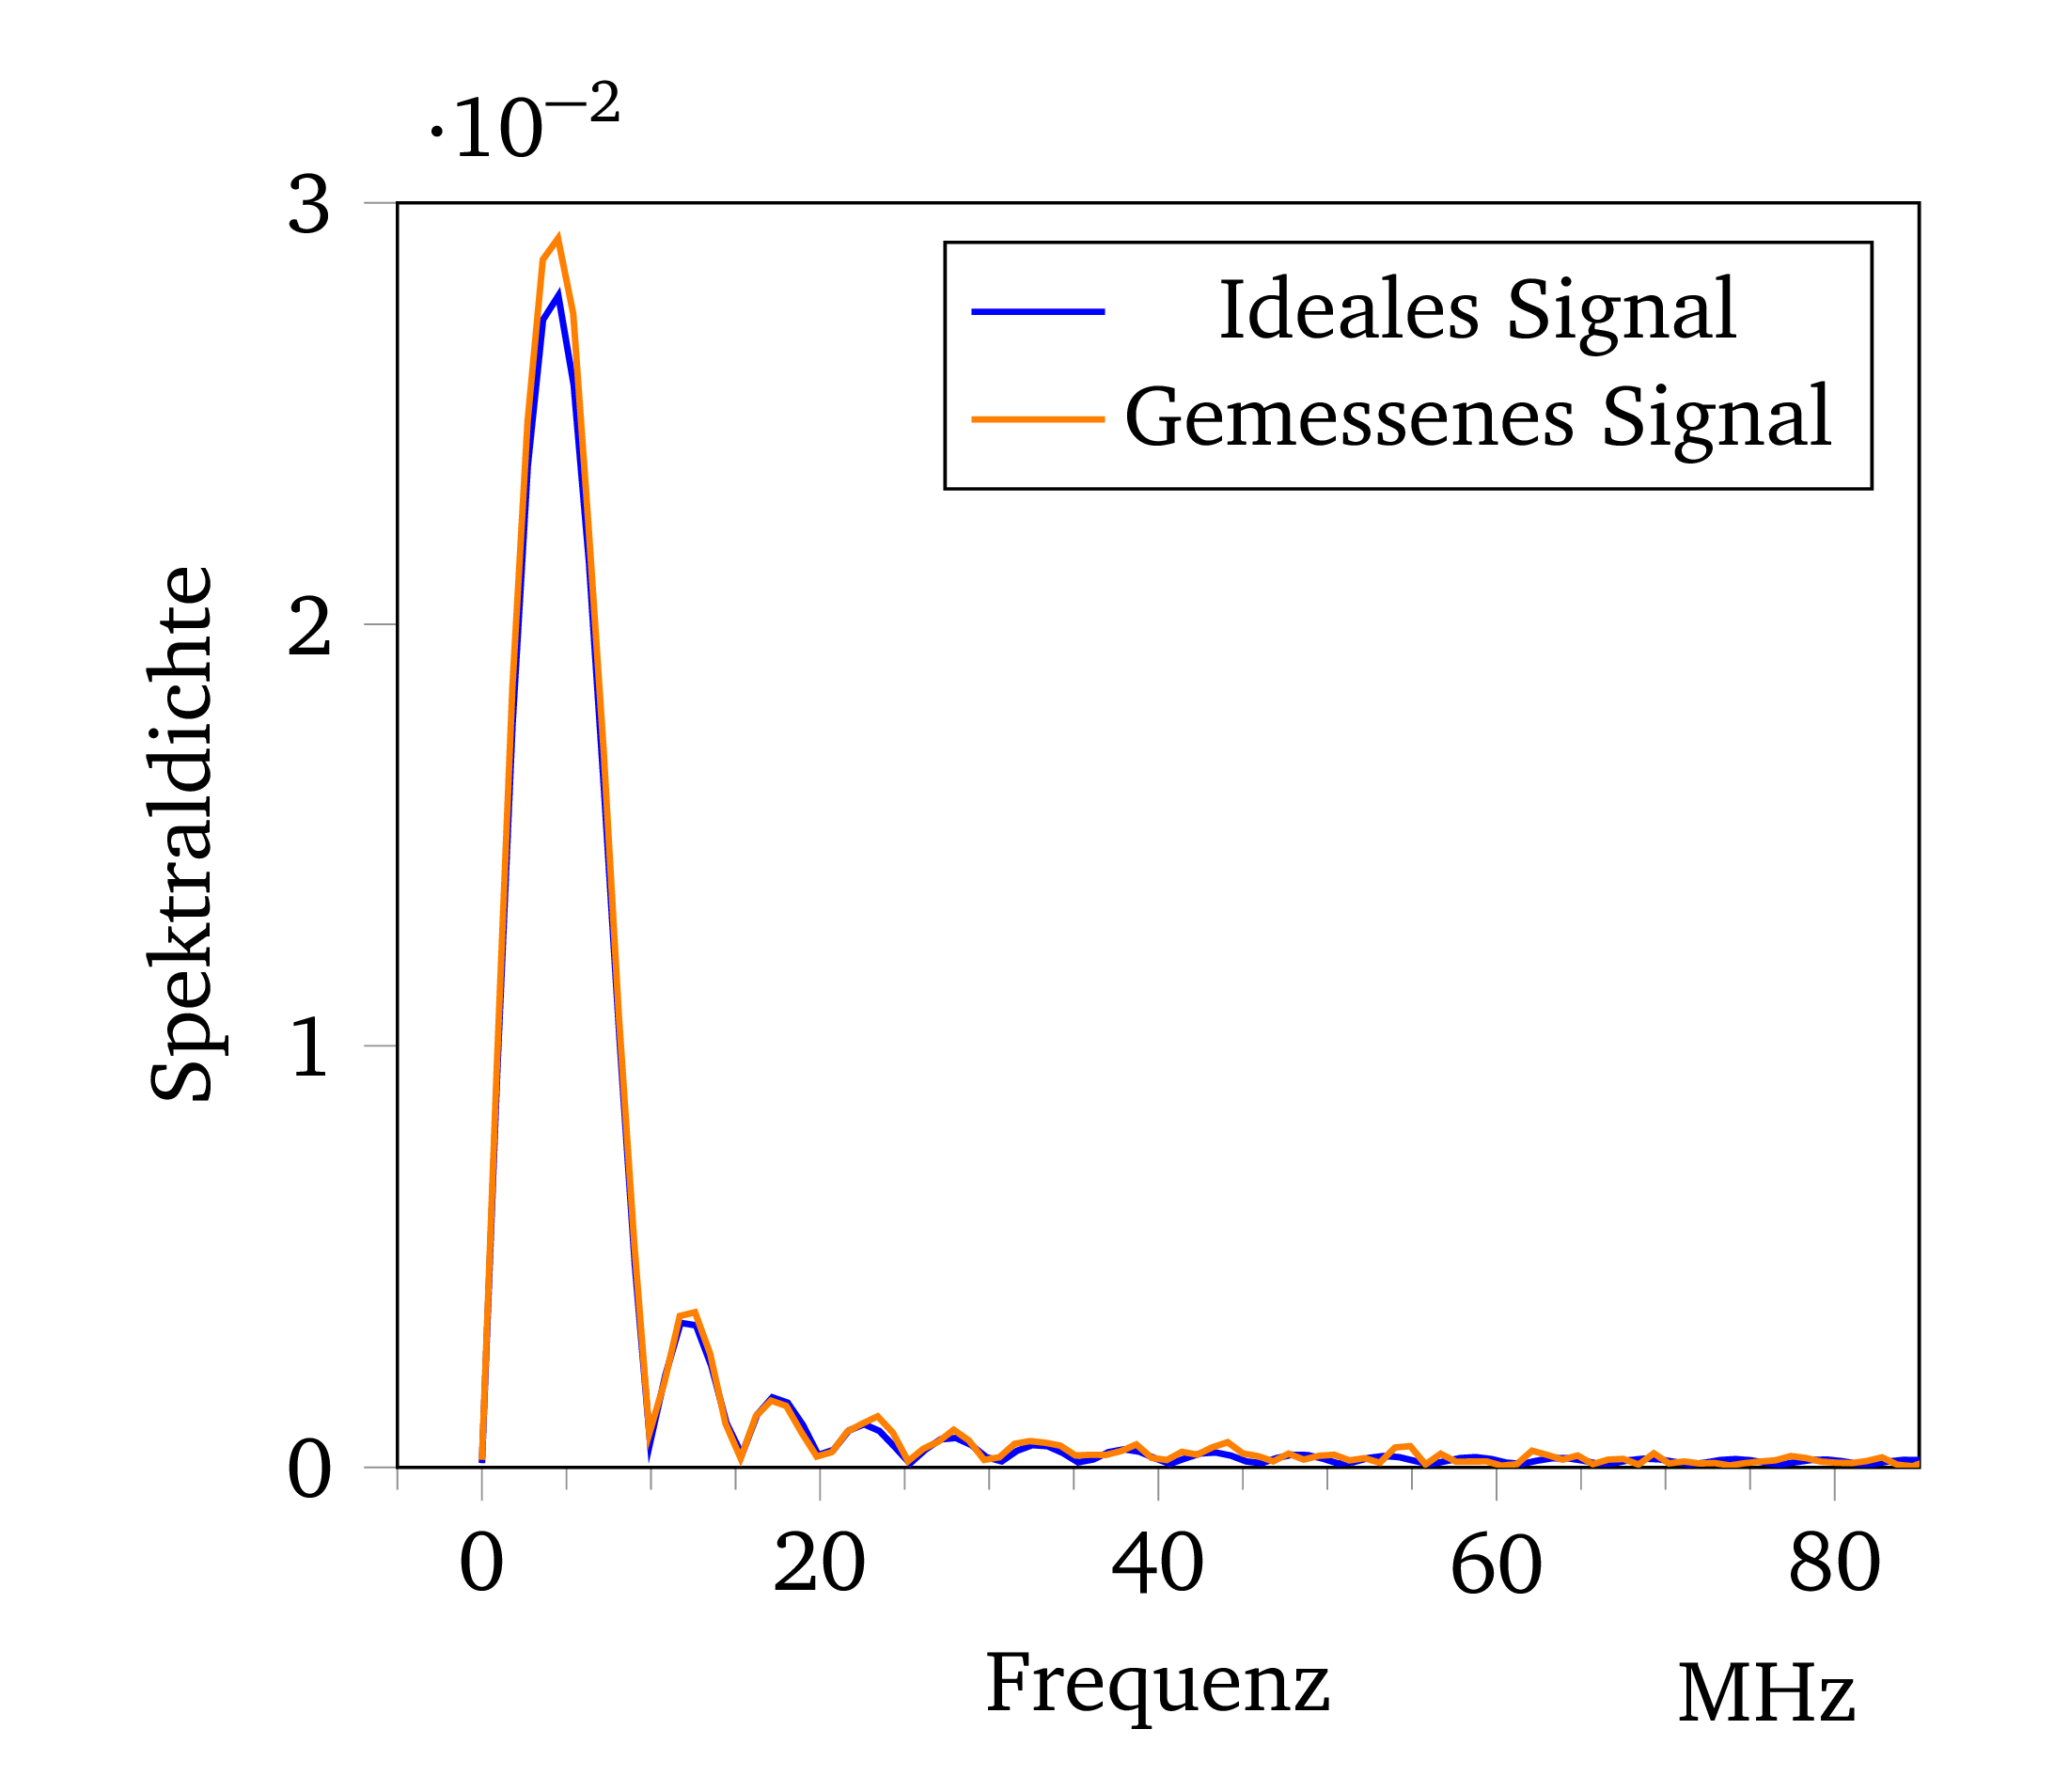
\includegraphics[scale=0.6]{slides/adjust_H/adjust_H_spectre.png}	
	}
\end{picture}	
}


\uncover<12>{
	\begin{picture}(0, -40)
	\put(145, 88){
		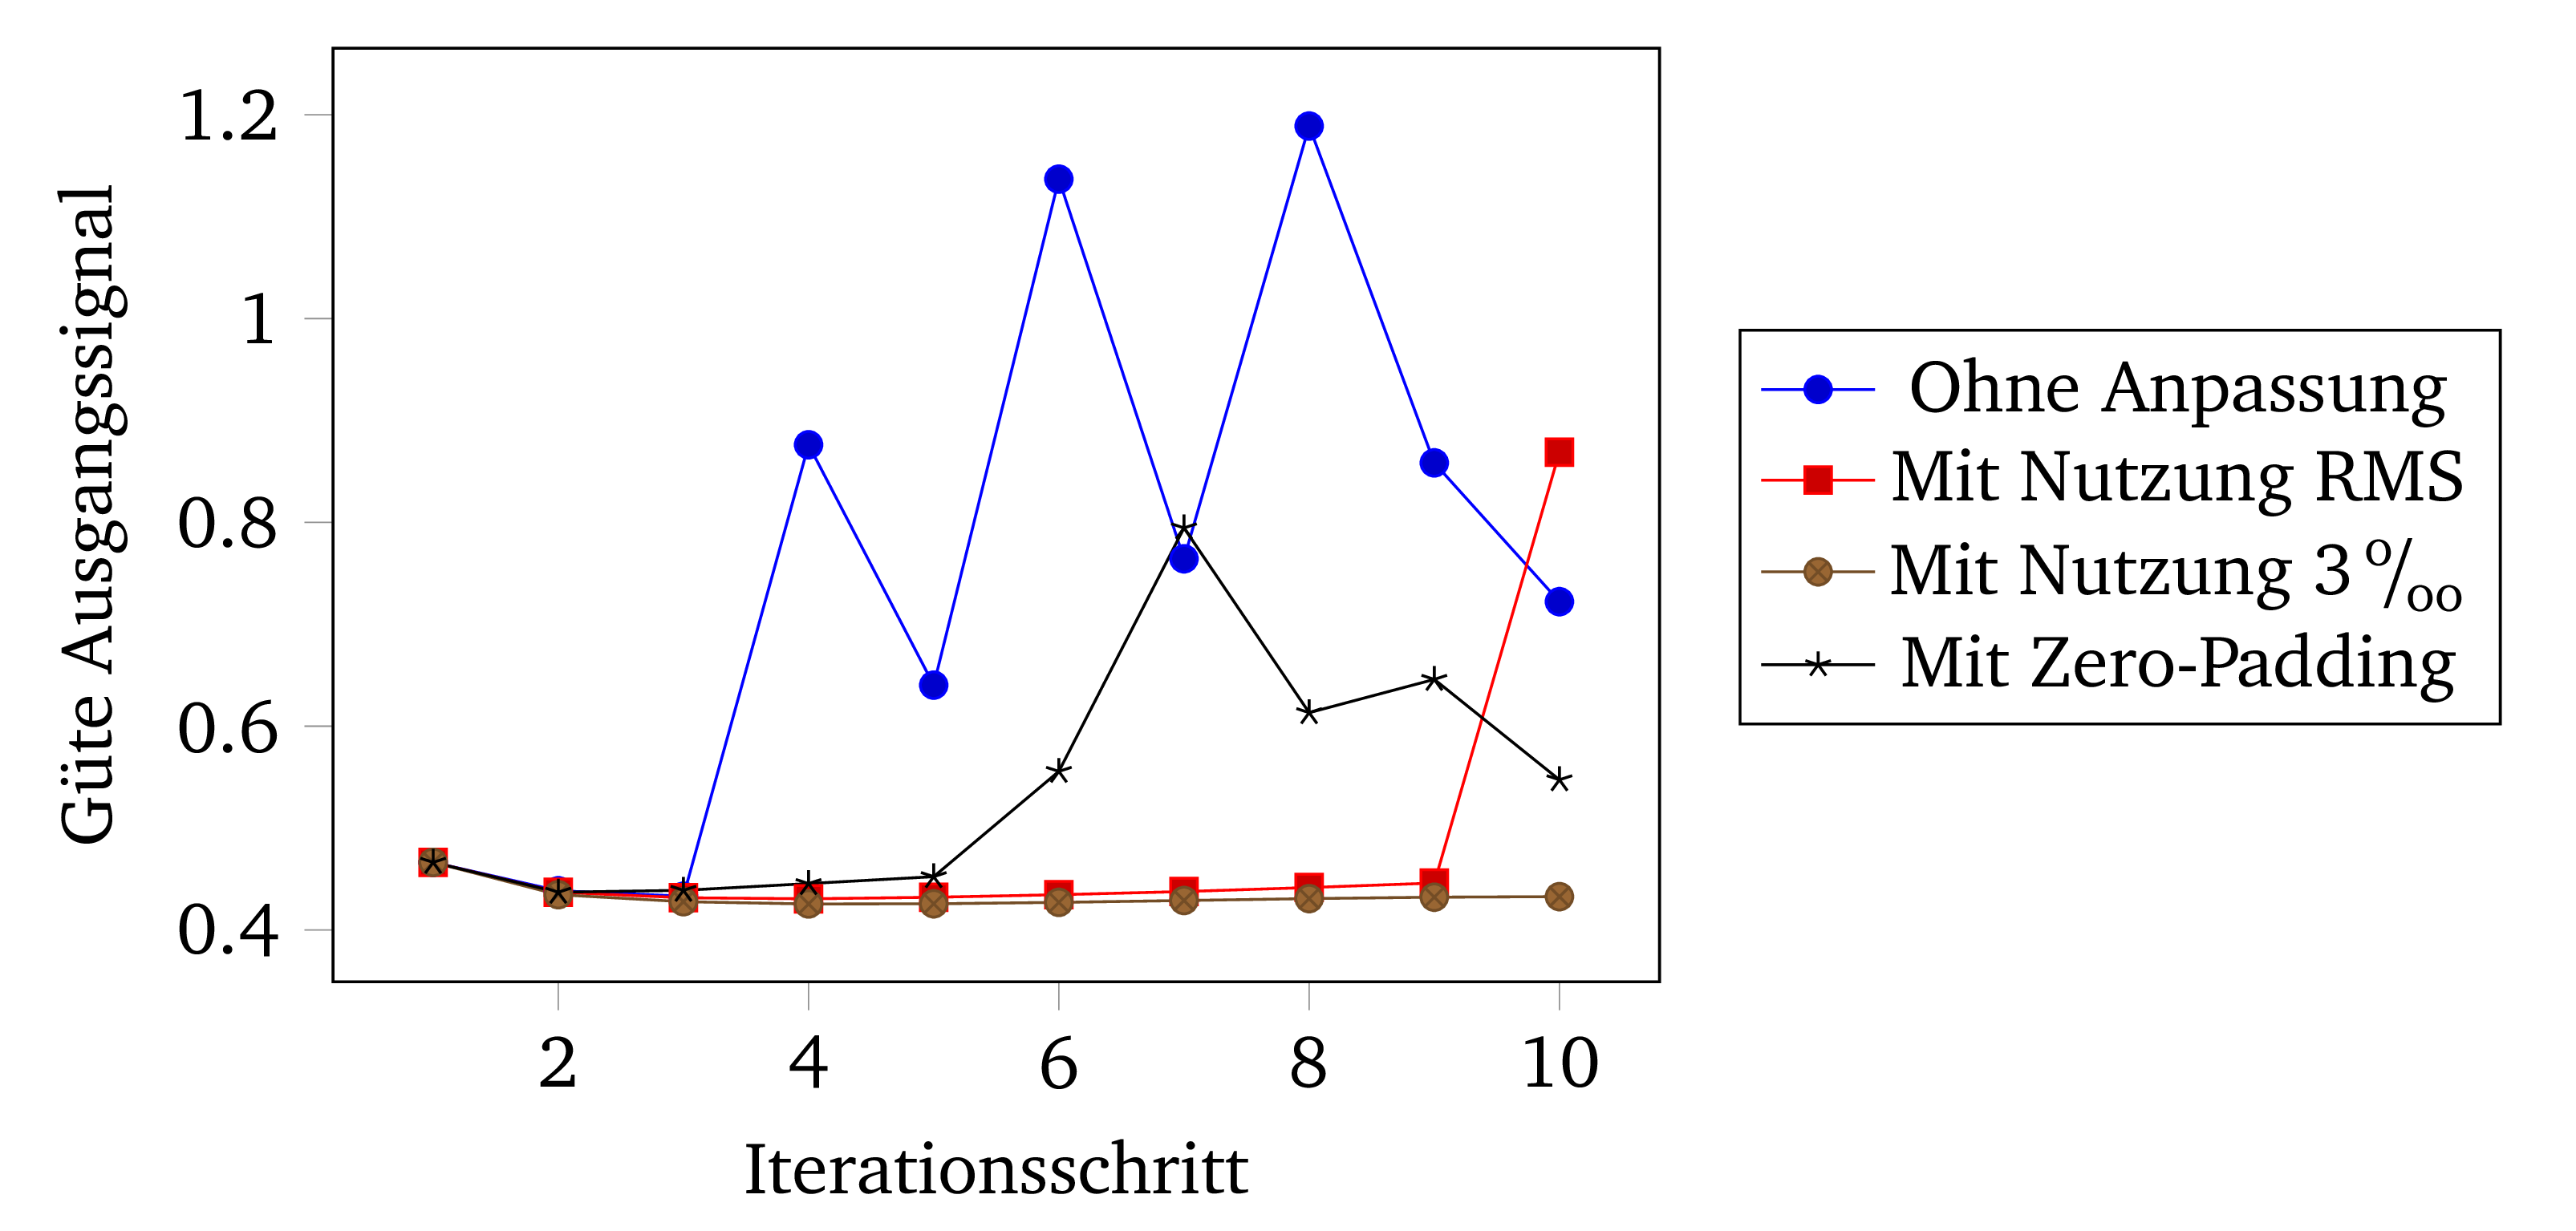
\includegraphics[scale=0.5]{slides/adjust_H/adjust_H_quality.png}	
	}
\end{picture}	
}

%
\uncover<13>{
	\begin{picture}(0, -80)
	\put(177, 70){
		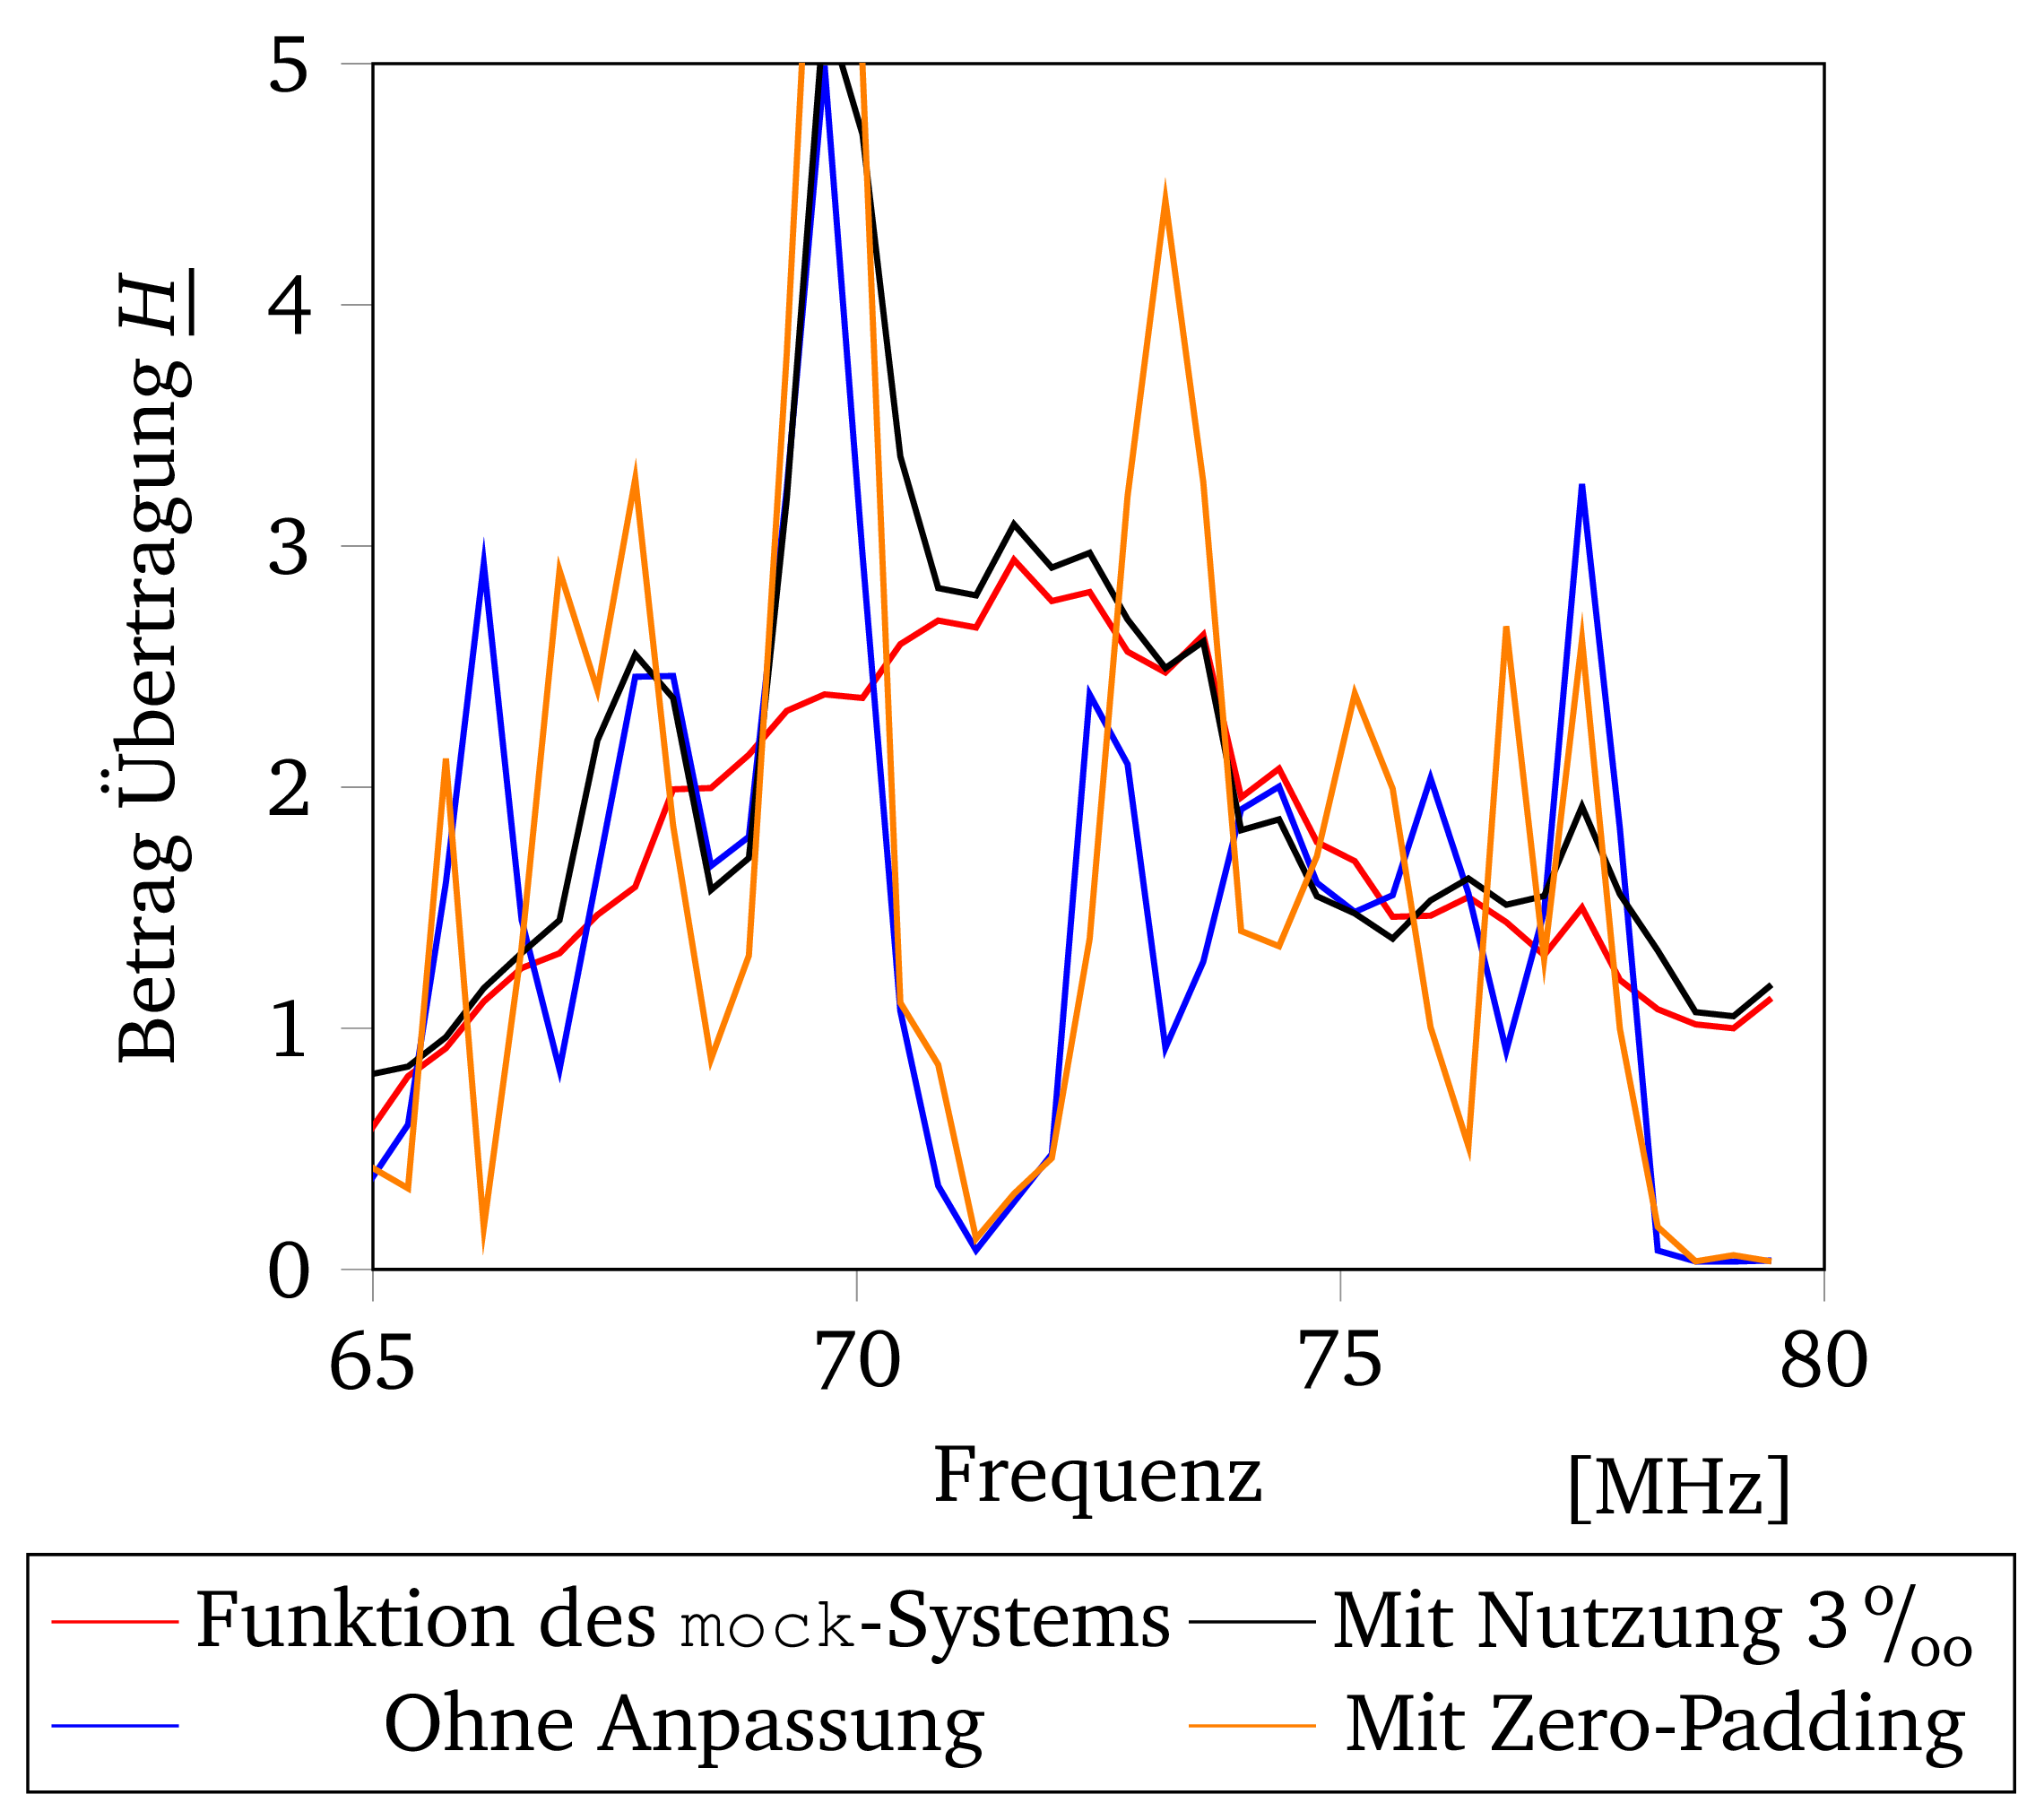
\includegraphics[scale=0.5]{slides/adjust_H/adjust_H_high_frequencies.png}	
	}
\end{picture}	
}


\end{frame}



